\documentclass{scrreprt}

\usepackage{aligned-overset}
\usepackage{amsmath}
\usepackage{amssymb}
\usepackage{bm}
\usepackage[shortlabels]{enumitem}
\usepackage{hyperref}
\usepackage[utf8]{inputenc}
\usepackage{multicol}
\usepackage{mathtools}
\usepackage{physics}
\usepackage{tabularx}
\usepackage{titling}
\usepackage{fancyhdr}
\usepackage{xfrac}
\usepackage{pgfplots}

\pgfplotsset{compat = newest}
\usetikzlibrary{intersections}
\usetikzlibrary{patterns}
\usepgfplotslibrary{fillbetween}

\author{Karsten Lehmann (Übungsgruppe 1)\\Mat. Nr 4935758}
\date{WiSe 2021/2022}
\title{Hausaufgaben Blatt 08\\Analysis - Grundlegende Konzepte}

\setlength{\headheight}{26pt}
\pagestyle{fancy}
\fancyhf{}
\lhead{\thetitle}
\rhead{\theauthor}
\lfoot{\thedate}
\rfoot{Seite \thepage}

\begin{document}
\paragraph{40. Beweisen Sie die folgenden Aussagen:}
\begin{enumerate}[(a)]
\item Es sei $M$ eine beliebige nicht-leere Menge und
  $f, g \colon M \to \mathbb{R}$ nach oben beschränkte Funktionen.
  Zeigen sie die Ungleichung
  \[
    \sup\qty{f(x) + g(x) \: {\Big |} \: x \in M}
    \leq
    \sup\qty{f(x) \: {\Big |} \: x \in M} +
    \sup\qty{g(x) \: {\Big |} \: x \in M}
  \]

  \subparagraph{Lsg.} Das Supremum ist als obere Schranke einer Menge größer
  oder gleich jedem Element der Menge.
  Sei nun $F \coloneqq \qty{f(x) \: {\Big |} \: x \in M}$ und
  $G \coloneqq \qty{g(x) \: {\Big |} \: x \in M}$.
  Dann $\sup F \geq f(x) \: \forall \: x \in M$ und
  $\sup G \geq g(x) \: \forall \: x \in M$.
  \begin{flalign*}
    \sup\qty{f(x) + g(x) \: {\Big |} \: x \in M}
    &\leq \sup\qty{\sup F + g(x) \: {\Big |} \: x \in M} \\
    &\leq \sup\qty{\sup F + \sup G \: {\Big |} \: x \in M} = \sup F + \sup G \\
    \overset{\text{Def. } F \text{ und } G}&=
    \sup\qty{f(x) \: {\Big |} \: x \in M} +  \sup\qty{g(x) \: {\Big |} \: x \in M}
  \end{flalign*}

\item Wir betrachten für $p, q \in \mathbb{R}$ mit $p, q \geq 1$ die Normen
  $\abs{\cdot}_p$ und $\abs{\cdot}_q$ auf dem $\mathbb{R}^n$.
  Zeigen Sie, dass diese Normen äquivalent sind.

  \subparagraph{Lsg.} Zwei Normen $\norm{\cdot}_1$ und $\norm{\cdot}_2$ auf
  $X$ heißen äquivalent, falls
  \[
    \exists \: \alpha, \beta > 0 \: \forall \: x \in X \colon
    \alpha \norm{x}_1 \leq \norm{x}_2 \leq \beta \norm{x}_2
  \]

  Für $x \in \mathbb{R}^n$ ist $\abs{x}_p =
  \qty(\overset{n}{\underset{i = 1}{\sum}} \abs{x_i}^p)^{\frac{1}{p}}$.

  Nach Beispiel 8.9 der Vorlesung ist
  \begin{flalign*}
    1 \cdot \norm{x}_{\infty} &\leq \norm{x}_p \leq \sqrt[p]{n} \norm{x}_{\infty} && \text{und} &&\\
    1 \cdot \norm{x}_{\infty} &\leq \norm{x}_q \leq \sqrt[q]{n} \norm{x}_{\infty} \\
    \Rightarrow \frac{1}{\sqrt[q]{n}} \norm{x}_q &\leq \norm{x}_{\infty} \\
    \Rightarrow \sqrt[p]{n} \norm{x}_{\infty} &\leq \sqrt[p]{n}\norm{x}_{q} \\
    \Rightarrow \frac{1}{\sqrt[q]{n}} \norm{x}_q &\leq \norm{x}_{\infty} \leq \norm{x}_p \leq \sqrt[p]{n} \norm{x}_{\infty} \leq \sqrt[p]{n}\norm{x}_{q} \\
    \Rightarrow \frac{1}{\sqrt[q]{n}} \norm{x}_q &\leq \norm{x}_p \leq \sqrt[p]{n}\norm{x}_{q}
  \end{flalign*}
\end{enumerate}

\newpage
\paragraph{41. Es sei $X \coloneqq \mathbb{R}_{> 0}$} und
$d \colon X \times X \to \mathbb{R}$ gegeben durch
\[
  d\qty\big(x, y) \coloneqq \abs{\frac{1}{x} - \frac{1}{y}}
  \qquad \qty\big(x, y \in X)
\]
Zeigen sie, dass $d$ eine Metrik auf $X$ ist.

\subparagraph{Lsg.} Eine Abbildung $d \colon X \times X \to \mathbb{R}$
heißt Metrik auf $X$, falls für alle $x, y, z \in X$ gilt
\begin{enumerate}[(a)]
\item $d\qty\big(x, y) = 0 \iff x = y$

  Es gilt $\abs{a} = 0 \iff a = 0$ und
  $\frac{1}{a} - \frac{1}{b} = 0 \iff a = b$.
\item $d\qty\big(x, y) = d\qty\big(y, x)$

  Nach Satz 5.5 der Vorlesung ist $\abs{a} = \abs{-a}$, also
  \[
    d\qty\big(x, y) = \abs{\frac{1}{x} - \frac{1}{y}}
    = \abs{-\qty(\frac{1}{x} - \frac{1}{y})}
    = \abs{\frac{1}{y} - \frac{1}{x}}
    = d\qty\big(y, x)
  \]
\item $d\qty\big(x, z) \leq d\qty\big(x, y) + d\qty\big(y, z)$

  \begin{flalign*}
    d\qty\big(x, z) \overset{\text{Def. } d}= \abs{\frac{1}{x} - \frac{1}{y}}
    &= \abs{\frac{1}{x} + 0 - \frac{1}{y}} \\
    &= \abs{\frac{1}{x} + \qty(\frac{1}{y} - \frac{1}{y}) - \frac{1}{z}} \\
    \overset{\text{Kommutativität}}&= \abs{\frac{1}{x} + \qty(-\frac{1}{y} +
      \frac{1}{y}) - \frac{1}{z}} \\
    \overset{\text{Assoziativität}}&= \abs{\qty(\frac{1}{x} + -\frac{1}{y}) +
      \qty(\frac{1}{y} - \frac{1}{z})} \\
    \overset{\text{Satz 5.5, $\bigtriangleup$-ungleichung}}&\leq
    \abs{\frac{1}{x} - \frac{1}{y}} + \abs{\frac{1}{y} - \frac{1}{z}} \\
    \overset{\text{Def. } d}&= d\qty\big(x, y) + d\qty\big(x, z)
  \end{flalign*}
\end{enumerate}



\newpage
\paragraph{42. Sei $X \coloneqq \mathbb{R}^2$.}
Skizzieren Sie

\begin{enumerate}[(a)]
\item für $p \in \qty\big{1, 2, \infty}$ die abgeschlossene Kugel vom Radius
  $r = 1$ um den Punkt $x = \qty\big(1, 1)$ bezüglich der $p$-Norm.

  \subparagraph{Lsg.}
  \begin{itemize}
  \item {\color{black!30!orange} $B_1\qty\big[(1, 1)]$ bezüglich der $1$-Norm.}
  \item {\color{black!30!green} $B_1\qty\big[(1, 1)]$ bezüglich der $2$-Norm.}
  \item {\color{black!30!blue!80} $B_1\qty\big[(1, 1)]$ bezüglich der $\infty$-Norm.}
  \end{itemize}
  \begin{tikzpicture}
    \begin{axis}[
        xmax = 2.2,
        xmin = -0.2,
        ymax = 2.2,
        ymin = -0.2]
      \draw[
        blue!20,
        fill = blue!10,
        very thick,
      ] (0,0) -- (0,2) -- (2,2) -- (2,0) -- cycle;
      \draw[
        green,
        fill = green!20,
        very thick,
      ] (1, 1) circle (1);
      \draw[
        orange,
        fill = orange!20,
        very thick,
      ] (0, 1) -- (1, 0) -- (2, 1) -- (1, 2) -- cycle;
      \draw[
        black,
        fill,
      ] (1, 1) circle (0.02);
      \node[black] at (1.2, 0.8) {$\qty\big(1, 1)$};
    \end{axis}
  \end{tikzpicture}

\item die abgeschlossene Kugel vom Radius $r_1 = \frac{1}{2}$ und $r_2 = 2$
  um den Punkt $x = \qty\big(0, 0)$ bezüglich der diskreten Metrik im
  $\mathbb{R}^2$.

  \subparagraph{Lsg.} Die diskrete Metrik ist definiert als
  $d\qty\big(x, y) \coloneqq \begin{cases}
    0 & x = y \\
    1 & x \ne y
  \end{cases}$.
  Somit ist
  \[
    B_{\frac{1}{2}}\qty\big((0, 0))
    = \qty{y \in \mathbb{R}^2 \: {\Big |} \: d\qty\big(x, y) < \frac{1}{2}}
    = \qty\big{\qty(0, 0)}
  \]
  und
  \[
    B_2\qty\big((0, 0))
    = \qty{y \in \mathbb{R}^2 \: {\Big |} \: d\qty\big(x, y) < 2}
    = \mathbb{R}^2
  \]
\end{enumerate}

\newpage
\paragraph{43. Untersuchen Sie, ob die Folgen} konvergent sind und berechnen Sie
gegebenenfalls deren Grenzwert:
\begin{enumerate}[(a)]
\item $\qty{\frac{1}{n^2}}_{n \in \mathbb{N}_{> 0}}$
  \subparagraph{Lsg.} Nach Beispiel 9.2 der Vorlesung ist
  $\lim_{n \to \infty} \frac{1}{n} = 0$.
  Weiter gilt nach Folgerung 9.15 der Vorlesung für zwei
  Folgen $\qty\big{a_n}, \qty\big{b_n}$ mit $a_n \to a, b_n \to b$,
  dass $a_nb_n \to ab$.

  \[
    \Rightarrow \lim_{n \to \infty} \frac{1}{n^2}
    = \lim_{n \to \infty} \qty(\frac{1}{n} \cdot \frac{1}{n})
    = \lim_{n \to \infty} \frac{1}{n} \cdot \lim_{n \to \infty} \frac{1}{n}
    = 0
  \]
\item $\qty{\binom{2n}{n}}_{n \in \mathbb{N}}$

  \subparagraph{Lsg.}
  \[
    \binom{2n}{n} = \frac{\qty\big(2n)!}{n!\qty\big(2n - n)!}
    = \frac{\qty\big(2n)!}{\qty\big(n!)^2}
    = \frac{\prod_{k = 1}^{n}\qty(n + k) \prod_{k = 1}^n k}{\prod_{k = 1}^n k \cdot \prod_{k = 1}^n k}
    = \frac{\prod_{k = 1}^{n}\qty(n + k)}{\prod_{k = 1}^n k}
    < n
  \]
  $\Rightarrow$ für jedes $\epsilon > 0$ und $x \in \mathbb{R}$ findet sich ein
  $n_0 \in \mathbb{N}$, so dass für alle $n > n_0$ gilt:
  $d\qty(\binom{2n}{n}, x) > \epsilon$.

  $\Rightarrow \binom{2n}{n}$ divergiert.
\end{enumerate}

\end{document}
